\documentclass[12pt]{article}\usepackage[]{graphicx}\usepackage[]{color}
% maxwidth is the original width if it is less than linewidth
% otherwise use linewidth (to make sure the graphics do not exceed the margin)
\makeatletter
\def\maxwidth{ %
  \ifdim\Gin@nat@width>\linewidth
    \linewidth
  \else
    \Gin@nat@width
  \fi
}
\makeatother

\definecolor{fgcolor}{rgb}{0.345, 0.345, 0.345}
\newcommand{\hlnum}[1]{\textcolor[rgb]{0.686,0.059,0.569}{#1}}%
\newcommand{\hlstr}[1]{\textcolor[rgb]{0.192,0.494,0.8}{#1}}%
\newcommand{\hlcom}[1]{\textcolor[rgb]{0.678,0.584,0.686}{\textit{#1}}}%
\newcommand{\hlopt}[1]{\textcolor[rgb]{0,0,0}{#1}}%
\newcommand{\hlstd}[1]{\textcolor[rgb]{0.345,0.345,0.345}{#1}}%
\newcommand{\hlkwa}[1]{\textcolor[rgb]{0.161,0.373,0.58}{\textbf{#1}}}%
\newcommand{\hlkwb}[1]{\textcolor[rgb]{0.69,0.353,0.396}{#1}}%
\newcommand{\hlkwc}[1]{\textcolor[rgb]{0.333,0.667,0.333}{#1}}%
\newcommand{\hlkwd}[1]{\textcolor[rgb]{0.737,0.353,0.396}{\textbf{#1}}}%
\let\hlipl\hlkwb

\usepackage{framed}
\makeatletter
\newenvironment{kframe}{%
 \def\at@end@of@kframe{}%
 \ifinner\ifhmode%
  \def\at@end@of@kframe{\end{minipage}}%
  \begin{minipage}{\columnwidth}%
 \fi\fi%
 \def\FrameCommand##1{\hskip\@totalleftmargin \hskip-\fboxsep
 \colorbox{shadecolor}{##1}\hskip-\fboxsep
     % There is no \\@totalrightmargin, so:
     \hskip-\linewidth \hskip-\@totalleftmargin \hskip\columnwidth}%
 \MakeFramed {\advance\hsize-\width
   \@totalleftmargin\z@ \linewidth\hsize
   \@setminipage}}%
 {\par\unskip\endMakeFramed%
 \at@end@of@kframe}
\makeatother

\definecolor{shadecolor}{rgb}{.97, .97, .97}
\definecolor{messagecolor}{rgb}{0, 0, 0}
\definecolor{warningcolor}{rgb}{1, 0, 1}
\definecolor{errorcolor}{rgb}{1, 0, 0}
\newenvironment{knitrout}{}{} % an empty environment to be redefined in TeX

\usepackage{alltt}
\usepackage[top=1.00in, bottom=1.0in, left=1.1in, right=1.1in]{geometry}
\renewcommand{\baselinestretch}{1.1}
\usepackage{graphicx}
\usepackage{natbib}
\usepackage{amsmath}
\bibliographystyle{..//refs/styles/besjournals.bst}
\def\labelitemi{--}
\parindent=24pt
\title{Supplement: Reconciling historic hypotheses regarding flower-leaf sequences in temperate forests for fundamental and global change biology}
\IfFileExists{upquote.sty}{\usepackage{upquote}}{}
\begin{document}
\maketitle
\subsection*{Methods}
\subsubsection*{Climate Change and FLS:}
To evaluate how FLS patterns have overtime in association with climate change we obtained phenological data for three European woody plant species with long term records of both flower (BBCH 60) and leafout phenology (BBCH 11) from the Pan European Phenological Database \citep{PEP725}. We restricted the data set to include only stations with more than 50 years worth of data. For each species, we modeled the number of days between flowering and leafing as a function of time, using a hinge model with 1980 as break point in accordance with climate change models of \citet(). \texitit{Lizzie do you have any citations for hinge models?} For each species, we displayed the pre-1980 mean and standard deviation of FLS offset and the post-1980 change in mean FLS offset that can be associated with climate change.
\subsubsection*{Case studies}
\indent\indent \textbf{MTSV and USFS:} For these two, categorical, species level case studies, we converted verbal descriptions of flower-leaf sequences into a binary response variable. For our more inclusive "functional" definition of hysteranthy which allows for overlap between phenophases, we included species entries with descriptions \textit{"flowers before the leaves"}, \textit{"flowers before or with leaves"} and textit{"flowers with leaves"} as hysteranthous. Our more restrictive "physiological" hysteranthy definition only included species described as \textit{"flowers before the leaves"} as hysteranthous.\\
\ident For modeling trait associates we chose three predictors to represent the three major FLS hypothesis; pollination syndrome, average flowering time and minimum precipitation levels across the species range. We obtained pollination syndrome and average flowering time information directly from the data sources and estimates of minimum precipitation from the USDA/NRCS Conservation plants characteristics \citep{USDA}. We coded pollination syndrome as binary, biotic- or wind-pollinated and assigned known ambophilous species in the genus \textit{Salix} to the ancestral, biotic-pollinated, state of angiosperms. We recorded flowering time as the average of the range of months of flowering reported in each data source.\\
\indent For these case studies, we modeled associations between hysteranthy and the trait predictors with logistical regressions in phylogenetic generalized linear modeling framework \citep{Ives2010} using the R package phylolm \citep{Ho2014}.Our models incorporated a published angiosperm phylogenetic tree \citep{Zanne2013} pruned to match the species list for each case study. Species found in the trait data set but not in the original phylogenetic tree were added to the pruned tree at the genus level root. In total 32 species were added to the generic roots for the MTSV data set and eight for the USFS data set. We visualize phylogentic patterning of FLS across the tree of each case study in figs. \ref{fig:S1-S3} and we report the phylogentic signal for each of the categorical case studies in (tab. \ref{tab:Table S1})
We ran the models with 599 bootstrapped re-sampling iterations for each data set \citep{Wilcox2000}. We re-scaled continuous predictors by subtracting the mean and dividing by two standard deviations to allow for a reasonable comparison of effect sizes between the binary and continuous predictors in this model \citep{Gelman2007}. To assess the phylogenetic structure of hysteranthous flowering, we used the Caper package \citep{Orme2013} to calculate a phylogenetic D statistic.\\
\indent \textbf{HF:} For each species in the HF data set, we calculated average time between flowering and leafing for each species. We approximated our "physiological" FLS characterization by recording the day between flower budburst and leaf budburst and our "functional" FLS categorization by recording the average number of days between flowers opening and leaves reaching 75\% of their full size. We also re-coded the HF continuous offset variables as binary response with positive values coded as hysteranthous and negative values as seranthous.\\ Our models used the same predictors as the MTSV and USFS datasets, except that we estimated the average flowering time directly from the HF dataset. For this case study, we use the the R package brms\citep{} to estimate the relationship between FLS and the predictors with  phylogenetically-weighted mixed model in a Bayesian framework.\\ 
\indent Though we make comparisons between all three inter-specific case studies, we had to use different modeling frameworks for the HF dataset because of its different data structure from the other two. MTSV and USFS data provide one response variable for each species while the HF data contains intra-specific differences in FLS, providing several different response values per species. Phylogenetic generalized linear models can only fit models with one response value per species, while brms over-fits these kinds of data \citep{} (Paul Burkrenker personal communication) and performs better on multi-response per species datasets like HF. We ran all datasets on each case study and while they do yield different absolute estimates, the patterns we found were consistent across each framework. Q: Should I show an all Bayesian plot and all pgls plot? \\
\indent \textbf{PEP 725:} For intra-specific analysis, we utilized phenological records from PEP725 stations in Germany with more than 10 years worth of flowering and leafout records \citep{PEP725} for species \textit{Alnus glutinosa},\textit{Fraxinus excelsior} and \textit {Betula pendula}. To test associations for population level variation in FLS and long term soil moisture, we obtained average August soil moisture raster grids 1991-2010 for Germany from the German Weather Service \citep{DWD}, and extracted soil moisture values at every cell. We then tested associations between average soil moisture at each PEP725 phenological station and average FLS for species \textit{Aesculus hippocastanum,} \textit{Alnus glutinosa},\textit{Fraxinus excelsior} and \textit {Betula pendula} using a Bayesian linear modeling framework with the brms package in R \citep{Burkner2018}. We also repeated the analysis with average April soil moisture data from the same time period and results were robust. To compare across case studies with different measures of for the water dynamics hypothesis  we report the effect of average soil moisture and minimum precipitation across range as ``water dynamics",\\
\indent Using same PEP725 species records, we used r-squared values extracted from linear models \citep{baseR} to evaluate whether FLS variation was primarily driven by flower or leaf timing variation (tab. \ref{tab:Table S2})\\


\section*{Supplimental Tables and Figures}
% latex table generated in R 3.6.0 by xtable 1.8-4 package
% Wed Oct 30 13:10:34 2019
\begin{table}[ht]
\centering
\begin{tabular}{l|l|l}
  \hline
Dataset & category & D \\ 
  \hline
MTSV & Functional & 0.08 \\ 
  MTSV & Physiological & 0.21 \\ 
  USFS & Functional & 0.65 \\ 
  USFS & Physiological & 0.11 \\ 
   \hline
\end{tabular}
\caption{\textbf{Table 1} D statistics for the inter-specific FLS datasets with different classifications of hysteranthy} 
\label{Test_table}
\end{table}


% latex table generated in R 3.6.0 by xtable 1.8-4 package
% Wed Oct 30 13:10:39 2019
\begin{table}[ht]
\centering
\begin{tabular}{lcc|c||cc|c}
  & \multicolumn{3}{c}{Flowering} & \multicolumn{3}{c}{Leafing}\\
 \hline
Species & Estimate & Std.error & R^2 & Estimate & Std.error & R^2 \\ 
  \hline
\textit{Alnus glutinosa} & -0.674 & 0.005 & 0.585 & 0.238 & 0.002 & 0.031 \\ 
  \textit{Fraxinus excelsior} & -0.534 & 0.004 & 0.417 & 0.241 & 0.003 & 0.052 \\ 
  \textit{Betula pendula} & -0.400 & 0.005 & 0.324 & 0.134 & 0.004 & 0.025 \\ 
  \textit{Aesculus hippocastanum} & -0.282 & 0.002 & 0.101 & 0.134 & 0.002 & 0.264 \\ 
   \hline
\end{tabular}
\caption{\textbf{The influence of intra-specific of flower and leaf phenological variation influence on quantitative FLS variability in four European tree species}. For the three hysteranthous species, flowering time is strong correlated with FLS variability while in the seranthous species 	extit{Aesculus hippocastanum} FLS is more tightly associated with leaf phenology} 
\label{Table2}
\end{table}



\pagebreak



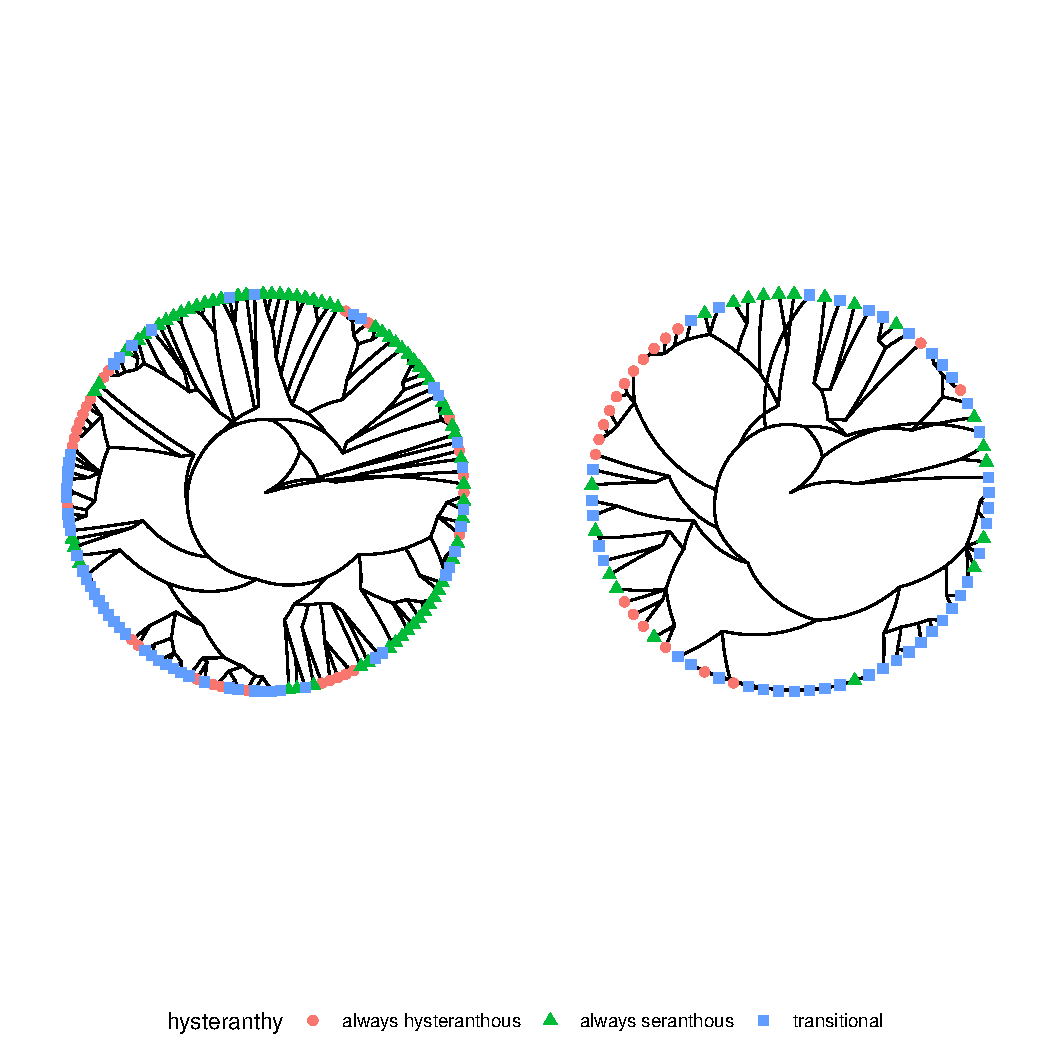
\includegraphics[width=\maxwidth]{figure/Code_chunk_Minimal_example3-1} 

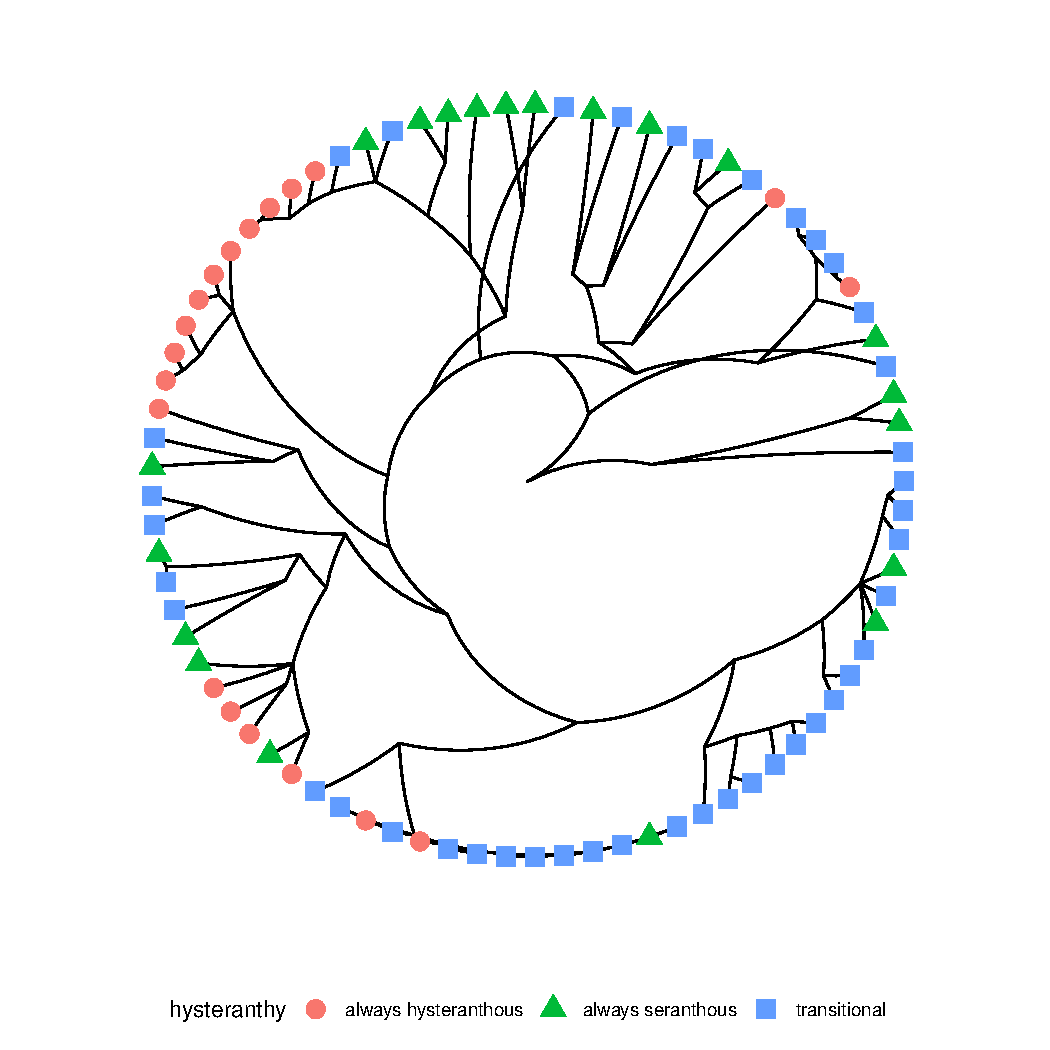
\includegraphics[width=\maxwidth]{figure/Code_chunk_Minimal_example3-2} 


\pagebreak 
    \caption{\textbf{Phylogenetic structure of FLS in MTSV.} As in the other two case studies, a large number of species get re-assigned to hysteranthy or seranthy (blue squares) depending on whether FLS is defined functionally (partial overlap between flowering and leafing allowed) or physiologically (no overlap between flowering and leafing allowed). This modeling choice dramatically alters FLS patterning across the tree, resulting in an unstable phylogentical signal for this trait.}
    \label{fig:Figure S1}
    \end{figure}
 

    \caption{\textbf{Phylogenetic structure of FLS in USFS.} As in the other two case studies, a large number of species get re-assigned to hysteranthy or seranthy (blue squares) depending on whether FLS is defined functionally (partial overlap between flowering and leafing allowed) or physiologically (no overlap between flowering and leafing allowed). This modeling choice dramatically alters FLS patterning across the tree, resulting in an unstable phylogentic signal for this trait.}
    \label{fig:Figure S2}
    \end{figure}
    

    \caption{\textbf{Phylogenetic structure of FLS in HF.} As in the other two case studies, a large number of species get re-assigned to hysteranthy or seranthy (blue squares) depending on whether FLS is defined functionally (partial overlap between flowering and leafing allowed) or physiologically (no overlap between flowering and leafing allowed). This modeling choice dramatically alters FLS patterning across the tree, resultinng in an unstable phylogentical signal for this trait.}
    \label{fig:Figure S3}
    \end{figure}




\end{document}
%o test for associations between FLS variability and inter-annual water availability we modeled the association between FLS and drought years from 2003-2010 using a bayesian linear modeling framework in BRMS\citep{}. Drought years were determined based on \citet{Ivits_2013}.
